\addcontentsline{toc}{subsection}{Hierarchy of Functions}


\begin{center}
    \textbf{\Huge Hierarchy of Functions}
\end{center}

\vspace{\stretch{1}}

\noindent We consider how fast different types of functions approach infinity. Here, assume that $c\in\mathbb{R}^+$ and $x\to\infty$.
\[...<\ln(\ln(x))<\ln(x)<x^{1/c}<x<x^c<c^x<x!<x^x<x^{x^x}<...\]

\begin{center}
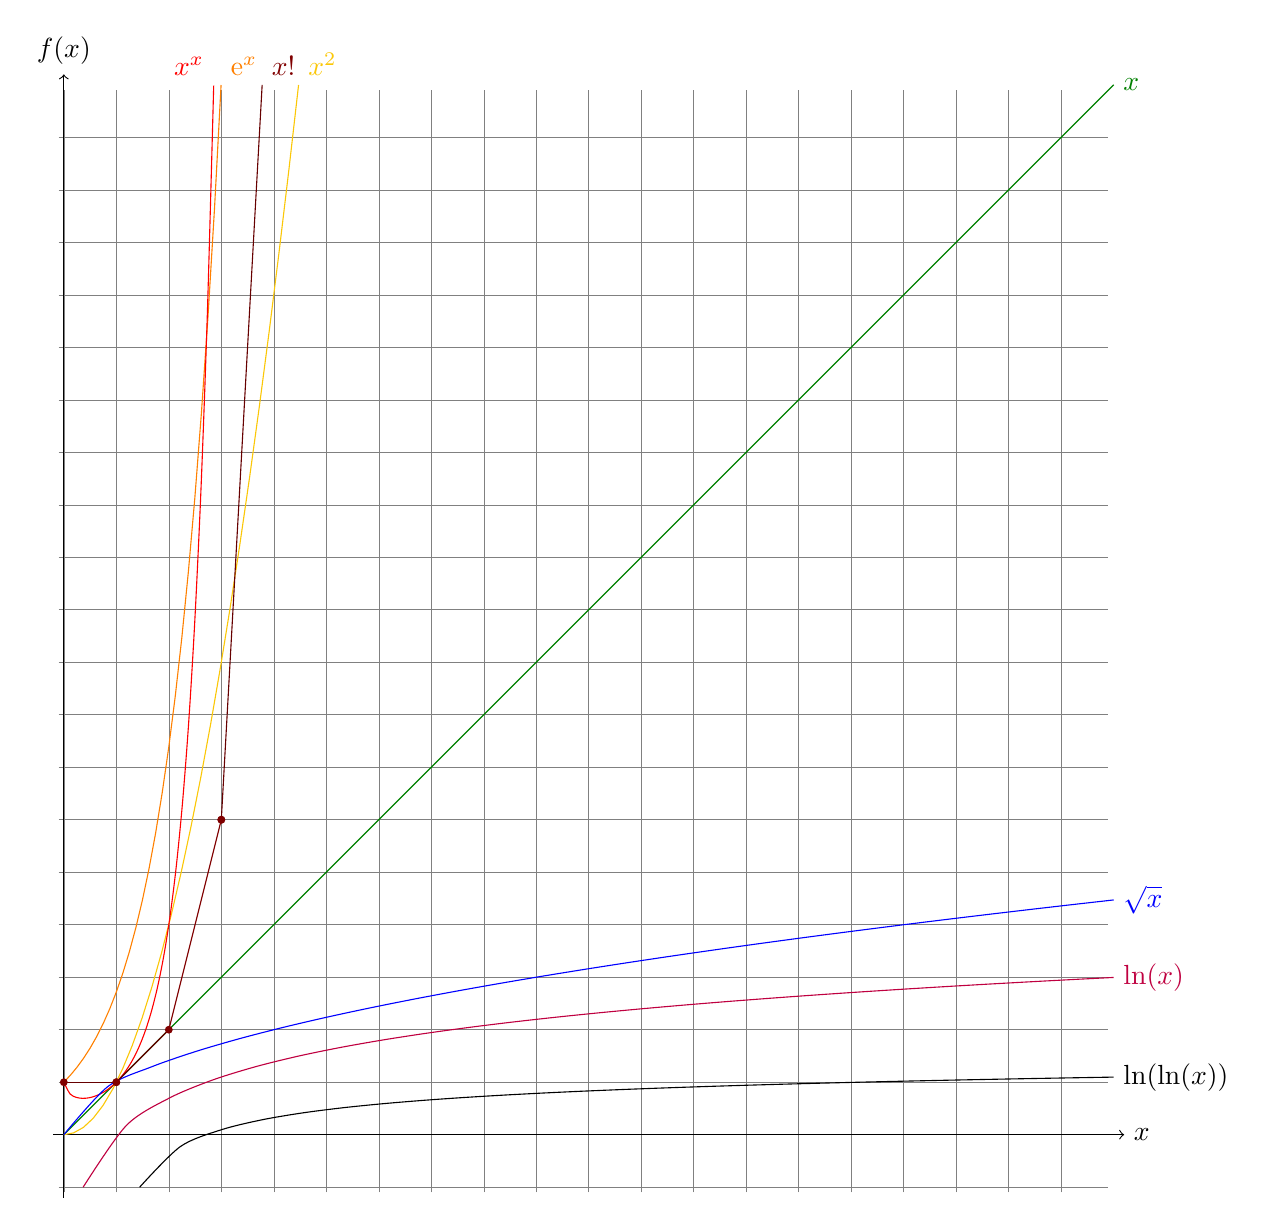
\begin{tikzpicture}[domain=0:20, xscale=2/3, yscale=2/3]
  \draw[very thin,color=gray] (-0.1,-1.1) grid (19.9,19.9);
  \draw[->] (-0.2,0) -- (20.2,0) node[right] {$x$};
  \draw[->] (0,-1.2) -- (0,20.2) node[above] {$f(x)$};
  \draw[color=black!50!green] plot (\x, \x) node[right] {$x$};
  \draw[color=orange, domain=0:ln(20)] plot (\x, {exp(\x) })
    node[above right] {$\mathrm e^{x}$};
  \draw[color=purple,domain=1/e:20, smooth] plot (\x,{ln(\x)}) node[right] {$\ln(x)$};
  \draw[color=yellow!60!orange, domain=0:sqrt(20)] plot (\x, {\x*\x}) node[above right] {$x^2$};
  \draw[domain=e^(1/e):20, smooth] plot (\x,{ln(ln(\x))}) node[right] {$\ln(\ln(x))$};
  \draw[color=red,smooth, domain=0:2.855330859]
  plot (\x,{\x^(\x)}) node[above left]{$x^x$};
  \draw[color=blue, smooth] plot (\x,{sqrt(\x)}) node[right]{$\sqrt{x}$};
  
  \draw[color=black!60!red] (0,1) node [circle,fill,color=black!50!red,inner sep=1pt]{} -- (1,1) node [circle,fill,color=black!50!red,inner sep=1pt]{};
  \draw[color=black!60!red] (1,1) node [circle,fill,color=black!50!red,inner sep=1pt]{} -- (2,2) node [circle,fill,color=black!50!red,inner sep=1pt]{};
  \draw[color=black!60!red] (2,2) [circle,fill,color=black!50!red,inner sep=1pt]{} -- (3,6) node [circle,fill,color=black!50!red,inner sep=1pt]{};
  \draw[color=black!60!red] (3,6) node [circle,fill,color=black!50!red,inner sep=1pt]{} -- (3.778,20) node [color=black!50!red, above right]{$x!$};
  
\end{tikzpicture}
\end{center}
\vspace{.2in}

\begin{center}
    The graph above shows some select examples of functions. Their growth helps us conceptualize certain limits involving their quotients.    
\end{center}

\vspace{\stretch{1}}

\newpage


